\subsection{Hemmelig kommunikation}
I dette afsnit vil der blive kigget på, hvordan man tidligere har anvendt kryptografi, for at skabe en basal forståelse for hvordan kryptering, eller kryptografi, er blevet til den teknologi der kendes i dag, samt hvilke fordele eller ulemper der kan tages til videre overvejelser.
\subsubsection{Oldtidens hemmelige kommunikation}
\begin{wrapfigure}{r}{0.53\textwidth}
    \vspace{-30pt}
    \begin{center}
        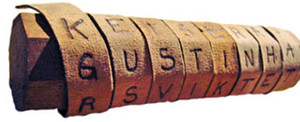
\includegraphics[width=0.75\linewidth]{Projectdoc/Problemanalyse/Illustrationer/scytale.jpg}
    \end{center}
    \caption{En spartansk scytale. Den hemmelige besked skrives på langs med cylinderen mens læderet er omviklet. Beskeden kan så først aflæses når læderet omvikles en lignende cylinder.}
    \vspace{-30pt}
    \label{fig:scytale}
\end{wrapfigure}
% Et af de første daterede kryptografi metoder blev opfundet og anvendt af spartanerne ca. 500 år før kristifødsel. \\
Et af de første daterede metoder indenfor hemmelig kommunikation blev opfundet og anvendt af spartanerne ca. 500 år før kristifødsel. \\
Denne metode "Den Spartanske scytale [Se Figur: \ref{fig:scytale}]" banede vejen for, hvad vi i dag kender, da denne opfindelse var en af de første, der ikke blot anvendte lokale metoder, så som sprog, men et faktisk værktøj og algoritme til at transponere kendte tekster til kode.\cite{PastCryptography}
%Den spartanske scytale var nemlig en cylinder, hvorom man viklede noget at skrive på, herefter skrev man sin besked på de enkelte sider, således når man fjernede cylinderen kunne man ikke forstå sammenhængen, før man havde en cylinder i samme størrelse.
%, dog findes også andre eksempler på mere avancerede anvendelse af værktøjer, så som kryptograferings maskinen "Enigma" fra Den Anden Verdens krig.\cite{PastCryptography}

\subsubsection{Hashings algoritmens forgænger}
Ca. 500 år efter den Spartanske scytale opfandt man i Rom, hvad der i dag er den mest kendte og brugte transponerings kryptografi "A-K Koden".
%\\A-K Koden går i alt sin simpelhed ud på, at man flytter alfabetet en vis grad, f.eks. i A-K ville "ABCD" skrives "KLMN", eller i A-S ville "ABCD" skrives "STUV".
\cite{TheSecretLanguage}\\
Denne krypterings metode har siden sin oprindelse været brugt i et større antal af nyopfundne metoder, 
%ikke kun pga. dens simpelthed og meget store aspekt af kombinationer, men også
mest grundet at den er grundlaget for alt fra simple algoritmer til de sværeste algoritmer. 
Faktisk kan man i flere af de nu-tids største datakrypterings algoritmer, også se en bassering på noget ligende en længere form af "A-K Koden", som man stadig udregner flere af. 
Dog er A-K Kodens største svaghed også dens udbredelse. Da denne kode i dag er kendt verden over, og efter anvendelse danner et ikonisk rod af usammenhængende bogstaver, der nemt ville genkendes som transformeret data, er denne metode også en af de først anvendte, i forskellige former, hvis en tredjepart skulle de-kryptere.

\subsubsection{Den nyere tids kryptografi}
Faktisk er A-K Koden så alment anvendt, at der kun findes et mindretal af nye og anderledes kryptografi former. Et eksempel på et sådant kunne dog være "Morse Koden" opfundet i 1836. Morse koden anvendte nemlig som andre former end kun tekst, men i stedet også lyd. 
%Lyden blev sendt gennem den datid revolutionerende telegraf og dens netledninger, også i vores tid kendt som telefonnettet.
\cite{Telegraphing} Denne nye idé at skjule ikke blot en handling, men også selve dens eksistens som støj, kan siges at have været en større mulighed, hvis ikke dens udførelse havde været så udbredt, at den i dag danner kendte ikoniske træk. F.eks. Vil de fleste i dag kunne genkende et "S.O.S".

\subsubsection{De legendariske steganografier}
Som nævnt i indledningen, så består emnet kryptologi af flere underkategorier. Den kategori der vil blive fokuseret mest på her, er steganografi. Dette omhandler metoder til at skjule selve eksistensen af en given besked, i stedet for at gøre indeholdet ulæseligt, som er hvad kryptografi.\cite{MeningOfSteganografi} Et eksempel på beskeder der er sikret med steganografi vil være de hemmelige signaler som der bruges af spioner i film. Et tilsyneladende tilfældigt symbol på et umiddelbart ligegyldigt sted, er blot en af de mange forskellige ting som kunne sende en besked sikkert frem. Alt dette vil foregå imens ingen andre vil opdage, at der overhoved var en form for kommunikation. Udenfor fiktion findes der også nogle eksempler på grupper som har udviklet systemer baseret på steganografi til at kommunikere internt.
%kommunikere internt. Fra kryptografiernes modsætningt  findes steganografi. Hvor kryptografi altid har været mere eller mindre alment kendt, er steganografier for det meste kun anvendt i mindre data baserede emner, og er derfor ikke udbredt eller kendt i lige så stort et omfang.
% Dog findes steganografi stadig i flere forskellige udformninger, og har blandt andet været anvendt til både handel, men også af f.eks. hjemløse.
\begin{figure}[H]
    \begin{subfigure}{0.5\textwidth}
    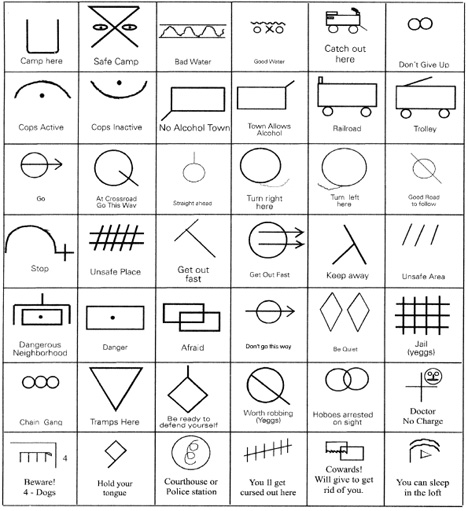
\includegraphics[width=0.9\linewidth, height=5cm]{Projectdoc/Problemanalyse/Illustrationer/hobo-glyphs-code.jpg} 
    \caption{The Hobo Code}
    \label{fig:hobocode}
    \end{subfigure}
    \begin{subfigure}{0.5\textwidth}
    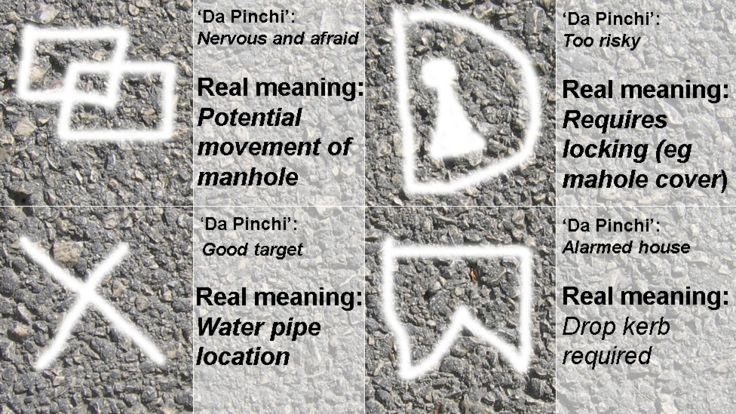
\includegraphics[width=0.9\linewidth, height=5cm]{Projectdoc/Problemanalyse/Illustrationer/BurglarsCode.jpg}
    \caption{Da Pinchi Code / The Burglars Code}
    \label{fig:burglarscode}
    \end{subfigure}
    \caption{To af de legendariske kryptografi metoder}
    \label{fig:legendscode}
\end{figure}
\noindent
Et kendt eksempel på en sådan steganografi metode kunne være "The Hobo Code [Se Figur: \ref{fig:hobocode}]", en bestemt del af kryptologien kendt, og anvendt, af hjemløse til at hjælpe hinanden med deres overlevelse\cite{TheHoboCode}. Disse beskeder er aldrig rigtigt blevet dateret, og ingen i dag kender derfor deres præcise oprindelse, men det vides dog stadig at denne kryptologiske metode har været anvendt i flere århundrede.\\ 
Foruden videnen om metodens eksistens gennem årene, vides også at der findes flere andre ligende afarter af denne kendte kode, såsom den nytidiske "Da Pinchi Code [Se Figur: \ref{fig:burglarscode}]". Denne kode bliver alment anvendt af konstruktions arbejdere, men siges også, efter historier, at have været anvendt af indbrudstyve eller andre kriminelle.\cite{DaPinchiCode}

\subsubsection{Anvendelsen}
Dette faktum at der findes flere steganografiske metoder, der ikke er særligt kendte, som man stadig kan anvende uden at f.eks. politiet aner uråd, giver et indtryk af at man ville kunne anvende ligende metoder i en nyere teknologi og derved muligvis opnå samme effekt. \\
Man prøver i dag ved alle tænkelige metoder at kryptere forbindelser på nettet, hashe data og oplysninger, eller lige frem at danne sikre VPN tunler mellem sender og modtager. Men alle disse har det tilfældes med A-K koden og Morsing, at de er kendte og synlige, og derfor på et eller andet tidspunkt vil deres sikkerhed blive brudt. Men de legendariske steganografiske metoder har alle den vigtige egenskab at de færreste ligger mærke til dem, selvom de befinder sig lige foran dem, midt på den offentlige gade. Disse egenskaber kunne, muligvis ved nærmere studie, blive anvendt til videregivelse af beskeder på F.eks. De åbne sociale medier, så som Facebook, der allerede er kendt for at tilbageholde alle informationer til videregivelse eller studie. Ved andre tilfælde, kunne denne metode måske endda også anvendes til udveksling af information på tværs af modstående lande, så som Rusland og USA.


% -------------------------
% Fra moderne kommunikation
% -------------------------

%\subsection{Moderne kommunikation}
%I det foregående afsnit blev udviklingen af hemmelig kommunikation gennemgået og en bestemt metode, steganografi, blev fremhævet som et muligt værktøj. I dette afsnit vil det blive undersøgt hvorfor og i hvilken udstrækning, at en ny type af hemmelig kommunikation skulle være nødvendig.
